\section{Method}
\label{sec:method}
\subsection{Algorithm}
The core of modeling current-reinforced random walks is that there are sources, sinks, nodes, particles and edges all organized within a graph representing a network. The fundamental idea is that sources send out information, sinks collect information and particles represent information. Edges are connections between sources, sinks and nodes and represent a path for the information to spread. Sources have a production rate, i.e the rate at which new particles are being injected into the system. Sinks have a removal rate, i.e. the rate at which particles are being removed from the system. Sources, sinks and nodes can all contain particles. For a system to have a viable solution for a minimized cost function the cumulative production rate of all the sources must be less than or equal to the cumulative removal rate of all the sinks, otherwise no flow equilibrium can be established.

There are some necessary parameters for this model to make sense. These parameters and their analogy in both electrical networks and ant trail networks are shown in Table \ref{tab:parameters}. How these parameters are used in the algorithm is in detail explained in Section \ref{sec:preparation} and \ref{sec:confirmation}.

\begin{table}[H]
\renewcommand{\arraystretch}{1.2}
\centering
\caption{Table shows the necessary parameters for the current-reinforced random walk modeling and their analogy in electrical networks and ant trail networks. $i$ denotes that the parameter corresponds to node $i$ and $ij$ denotes that the parameter corresponds to the edge between node $i$ and node $j$.}
\label{tab:parameters}
\begin{tabular}{ c | c | c }                       
	\textbf{Parameter} & \textbf{Electrical network} & \textbf{Ant trails} \\
	\hline
	$l_{ij}$ & length in space & length in space \\
	\hline
	$N_{i}$ & number of electrons & number of ants \\
	\hline	
	$P_{i}$ & potential & inverse flowness \\
	\hline
	$I_{ij}$ & current & flow of ants \\
	\hline
	$\bar{I}_{ij}$ & expected value of current & mean flow of ants \\
	\hline
	$D_{ij}$ & conductivity & pheromone concentration \\
	\hline
	$C_{i}$ & capacitance & total pheromone density \\
	\hline
	$q$ & reinforcement intensity & pheromone drop rate \\
	\hline
	$\lambda$ & conductivity decrease rate & pheromone evaporation rate \\
\end{tabular} 
\end{table}

The underlying algorithm for the current-reinforced random walk can be described by some key steps. At each time step the algorithm can be divided into two parts, one preparation part and one confirmation part. The reason for this i because synchronization is needed when implementing the algorithm in parallel. This is further explained in Section \ref{sec:parallel}. An outline of this algorithm is shown in Algorithm \ref{alg:outline}.

%The preparation step contains updating of the mean flow $\bar{I}_{ij}$, needed in order to randomize a new number of particles to move from one node to another i.e. the flow $I_{ij}$, and also contains the actual update of the flow $I_{ij}$.
%
%The confirmation step begins with updating the the conductivity $D_{ij}$. The conductivity is needed in order to calculate the new capacitance $C_{i}$. The new number of particles $N_{i}$ within a node is calculated from the previous number of particles and the flow $I_{ij}$ generated in the preparation step. The calculation of $N_{i}$ and $C_{i}$ are not dependent on each other and can be done in any order. The final stage in the confirmation step is the calculation of the potential $P_{i}$, which depends on $C_{i}$ and $N_{i}$. When this is finished the next time step can be started.

{
\vspace{1em}
\begin{algorithm}[H]
Preparation:\\
\ForEach{node}{
	\ForEach{neighbor}{
		update mean flow $\bar{I}_{ij}$\;
		randomize new flow $I_{ij}$\;
	}
}
\ \\
Confirmation:\\
\ForEach{node}{
	\ForEach{neighbor}{
		update conductivity $D_{ij}$\;
	}
	calculate capacitance $C_{i}$ and update number of particles $N_{i}$\;
	calculate potential $P_{i}$\;
}
\caption{Outline of the algorithm used in the current-reinforced random walks in \cite{Sumpter}.}
\label{alg:outline}
\end{algorithm}
\vspace{1em}
}

\subsubsection{Preparation}
\label{sec:preparation}
The preparation begins with each node calculating the mean flow $\bar{I}_{ij}$ to each of its neighbors as

\begin{equation}
\bar{I}_{ij} = \frac{(N_i - N_j)D_{ij}}{l_{ij}},
\end{equation}

 \noindent from which it can be seen that the mean flow depends on the conductivity of each edge, $D_{ij}$, which is 	initialized at and kept at or above some minimal value. The actual flow along the edge $ij$ can then be calculated as

\begin{equation}
I_{ij} = \text{Poi}(|\bar{I}_{ij}|\Delta t).
\end{equation}

In terms of implementation, it is important that nodes that are connected to the same edge agree on the same number of particles to transfer. This is ensured by allowing only the node with a larger number of particles to randomize the value and then both nodes use that value when updating the number of particles. The order of randomizing the number of particles to move to each neighboring node is uniformly randomized at each time step for each node. This means that there is no bias in choosing flow calculation order, i.e. no node will always have its number of particles randomized first. Since it is also important to ensure that there never are fewer than zero particles at a node the number of particles will continuously decrease while randomizing the amount of particles to move. When a node has a smaller number of particles than a given neighbor, the node always calculates the flow to that neighbor as zero and then waits for the neighboring node to tell it how many particles should be moved. The flow should theoretically be symmetric, but since only one node has randomized a value, and the other has set it to zero, the flow is not symmetric in this implementation. After all nodes have calculated and stored $\bar{I}$ and $I$, the preparation step is finished.

\subsubsection{Confirmation}
\label{sec:confirmation}
At the beginning of the confirmation part, all the data regarding how many particles will move along each edge is available. And so each node begins by updating the conductivity, which is calculated as

\begin{equation}
D_{ij}(t + \Delta t) = D_{ij}(t) + q|\bar{I}|^\mu - \lambda D_{ij}(t)\Delta t,
\end{equation}

 \noindent where $q$ is the reinforcement intensity caused by per unit flow, $\mu$ is the path maintenance parameter, $\lambda$ is the conductivity decay parameter and $\Delta t$ is the time step. If $\mu$ is set to one the current-reinforced random walk is linear and will converge to the same solution every time. If $\mu$ is set to a value greater than one the current-reinforced random walk becomes non-linear and will not converge to the same solution every time that a system is simulated. In the algorithms linear state it optimizes the path length for each individual path from the sources to the sinks, i.e it minimizes the cost function

\begin{equation}
\sum_{j \in \text{Neighbors}(i)} l_{ij} \bar{I}_{ij},
\end{equation}

 \noindent where $l_{ij}$ is the edge length between node $i$ and $j$ and $\bar{I}_{ij}$ is the corresponding mean flow of particles. This means that the algorithm always will find the shortest path through the graph. When utilizing the algorithm in its non linear state a combination of path length and path maintenance is optimized. No cost function for the non linear case has analytically yet been found. A proposition for such a cost function is suggested in \cite{Sumpter}. 

After the conductivity is updated the number of particles and the capacitance can be calculated. The new number of particles is calculated as

 \begin{equation}
 N_i(t + \Delta t) = N_i(t) + \sum_{j \in \text{Neighbors}(i)} \left( I_{ji} - I_{ij} \right).
 \end{equation}

 \noindent The capacitance is calculated as 

 \begin{equation}
 C_i = \sum_{j \in \text{Neighbors}(i)} D_{ij}/l_{ij},
 \end{equation}
 
 \noindent and finally the potential is calculated as
 
 \begin{equation}
 P_i = \frac{N_i}{C_i}.
 \end{equation}
 
 \noindent When this is done the time step is finished and the next time step can be started.

\subsection{Implementation and parallelism} 
\label{sec:parallel}
In order to achieve good performance it is important to implement the algorithm within a high performance environment. An ideal programming language for applications with high performance requirements is \texttt{C++}, which gives the programmer good control over optimizations and provide support for low level memory manipulation. It is also a good language for object oriented programming, which makes application design much easier. Other good features of \texttt{C++} is that it has generic and imperative programming features and is also very well suited for implementing parallel applications, both when utilizing smaller shared memory models and big scale message passing systems. Since the simulations done in \cite{Sumpter} were implemented serially in Matlab \texttt{C++} is a very suitable language of choice for significantly increasing the performance and taking the simulations into the parallel realm.

The algorithm shown in Algorithm \ref{alg:outline} can be parallelized in each of the outer loops, with synchronization after each preparation step and after each confirmation step. The synchronizations are necessary since the update of the conductivity depends on the flow from the neighboring nodes and since the update of the mean flow depends on the potential of the neighboring nodes. Therefore, a node and its neighbors must all have done the necessary steps before moving on to the confirmation part. So strictly speaking, global synchronization is not necessary, i.e. all nodes must not wait for all nodes to finish the preparation part, a node must only wait for its neighbors to finish. However, global synchronization is much simpler implementation-wise and may not be slower since it avoids complicated synchronization patterns.

The actual implementation uses OpenMP to parallelize the computations, each of the outer for-loops in Algorithm \ref{alg:outline} is parallelized using the directive \texttt{\#pragma omp parallel for}, which implicitly uses static scheduling where each core is assigned the same number of nodes. This is not perfectly matched with the graph partitioning method that is used (see section \ref{sec:graph_part}), but should only lead to slightly more implicit communication between cores.

{
\vspace{1em}
\begin{algorithm}[H]
Preparation\\
Sync\\
Confirmation\\
Sync\\
\caption{Outline of the parallel version of the algorithm showed in Algorithm \ref{alg:outline}.}
\label{alg:parallel}
\end{algorithm}
\vspace{1em}
}

\subsection{Graph partitioning}
\label{sec:graph_part}
When utilizing multicore systems it is important to minimize memory invalidation, i.e. communication between cores, in order to get good performance. This can be done in numerous ways but when working with graphs a natural way of minimizing memory invalidation is to partition the graph. Partitioning the graph must be done in a clever way so that there are as few edges as possible connecting nodes belonging to different cores. A rigorous way of partitioning graphs is presented in \cite{Lasalle}. A schematic view of such a graph partitioning is shown in Figure \ref{fig:partitioning}. Graph partitioning is great subject for research, hence many softwares for partitioning graphs in good ways have been developed through the years. The particular software used for the graph partitioning in this project is METIS. 

\begin{figure}[H]
\centering
\begin{subfigure}[b]{0.48\textwidth}
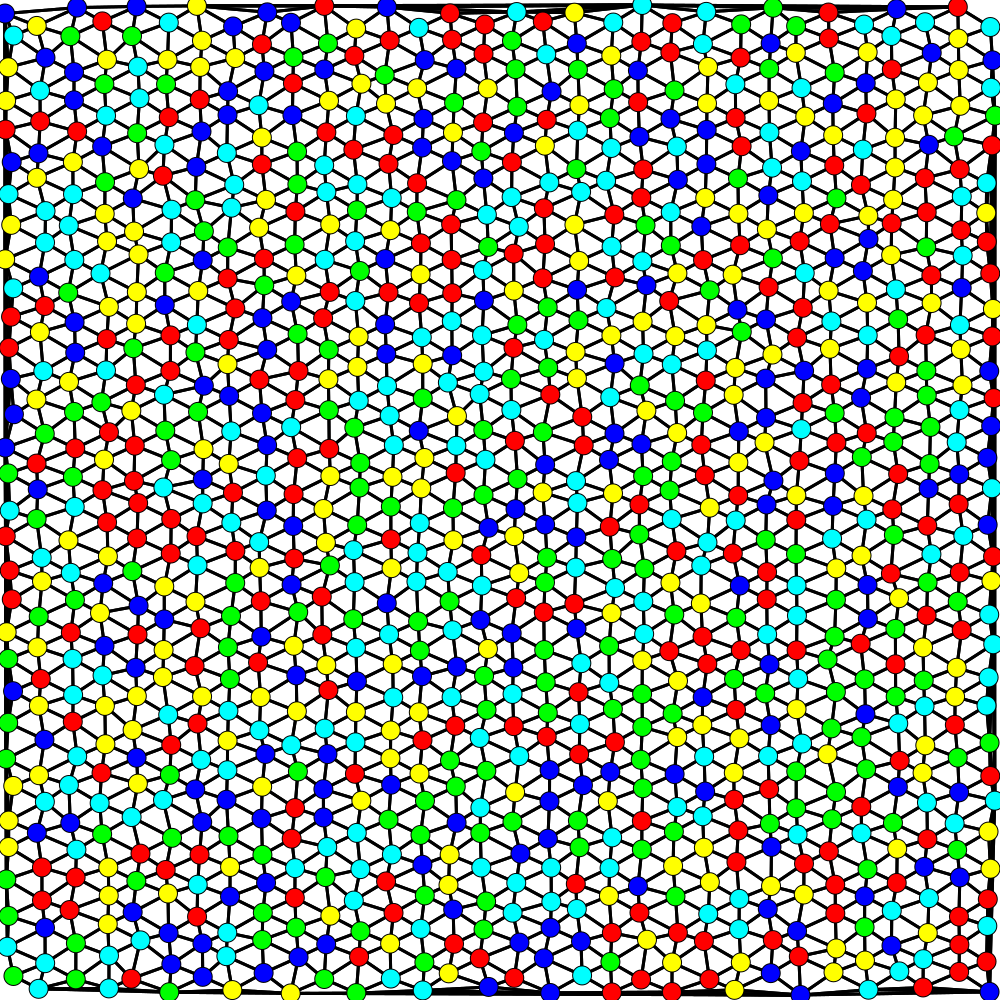
\includegraphics[width=\textwidth]{img/partitioning_false.png}
\caption{Non-partitioned graph.}
\end{subfigure}
~
\begin{subfigure}[b]{0.48\textwidth}
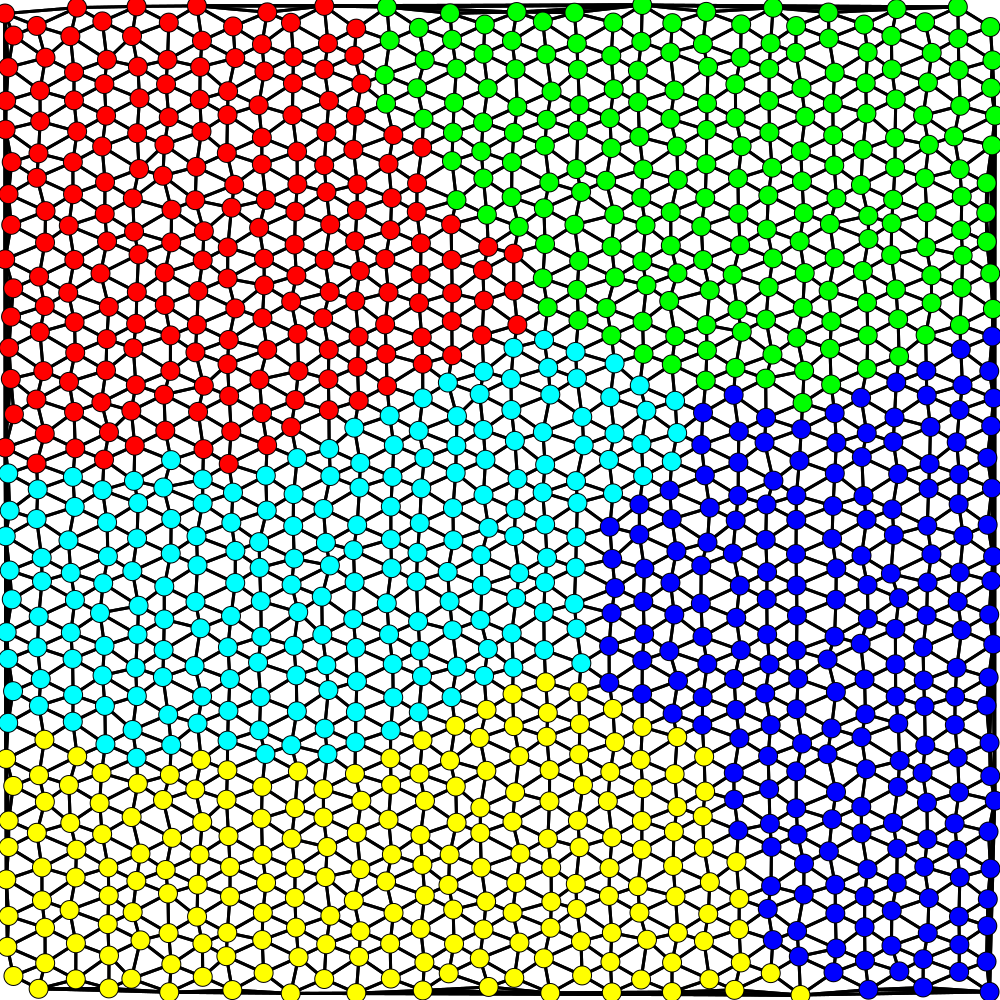
\includegraphics[width=\textwidth]{img/partitioning_true.png}
\caption{Partitioned graph.}
\end{subfigure}
\caption{Figure shows the difference in number of edges connecting nodes belonging to different cores for non-partitioned and partitioned graphs. Each color represents nodes belonging to different threads. The partitioned graph was partitioned with METIS.}
\label{fig:partitioning}
\end{figure}
